\documentclass[a4paper,12pt]{article}
   % Packages and definitions:
   % {
      \usepackage{float}
      \usepackage[english]{babel}
      \usepackage[utf8]{inputenc}
      \usepackage{amsmath}
      \usepackage{amssymb}
      \usepackage{color}
      \usepackage{subcaption}
      \usepackage{booktabs}
      \usepackage{tikz}
      \usepackage{multirow}
      \usetikzlibrary{decorations.pathreplacing}
      \usepackage{graphicx,epstopdf}
      \usepackage{cleveref}
      \usepackage{collcell} % loads array
      \usepackage{listings}
      \newcolumntype{m}{>{$} r <{$}}
      \newcolumntype{u}{>{$[\collectcell\si} l <{\endcollectcell]$}}
      \newcommand{\approxtext}[1]{\ensuremath{\stackrel{\text{#1}}{=}}}
      \newcommand{\matr}[1]{\mathbf{#1}}
      \newcommand{\partt}[2]{\ensuremath{\dfrac{\d {#1}}{\partial {#2}}}}
      \renewcommand{\d}[1]{\ensuremath{\operatorname{d}\!{#1}}} % non-italized differentials
      \newcommand{\h}[0]{\ensuremath{\hbar}} % hbar
      \newcommand{\qed}[0]{\ensuremath{\tag*{$\square$}}} % QED square
      \def\changemargin#1#2{\list{}{\rightmargin#2\leftmargin#1}\item[]}
      \let\endchangemargin=\endlist 
      \usepackage{amsthm}
      \theoremstyle{plain}
      \newtheorem{thm}{theorem} % reset theorem numbering for each chapter
      \theoremstyle{definition}
      \newtheorem{defn}[thm]{definition} % definition numbers are dependent on theorem numbers
      \newtheorem{exmp}[thm]{example} % same for example numbers
      \bibliographystyle{natbib}
      \renewcommand{\theequation}{\thesection.\arabic{equation}}
      \newcommand{\ts}{\textsuperscript} 

      \definecolor{dkgreen}{rgb}{0,0.6,0}
      \definecolor{gray}{rgb}{0.5,0.5,0.5}
      \definecolor{mauve}{rgb}{0.58,0,0.82}

      \lstset{frame=tb,
        language=Java,
        aboveskip=3mm,
        belowskip=3mm,
        showstringspaces=false,
        columns=flexible,
        basicstyle={\small\ttfamily},
        numbers=none,
        numberstyle=\tiny\color{gray},
        keywordstyle=\color{blue},
        commentstyle=\color{dkgreen},
        stringstyle=\color{mauve},
        breaklines=true,
        breakatwhitespace=true,
        tabsize=3
      }
% }
\title
{
	\textbf
	{
   Don't go sick to Malta:\\
   How a disease would spread in the EU28 zone
   }
}

\author{Henrik Åhl\\
\small{in collaboration with Denhanh Huynh}}
\date{\today}

\begin{document}
\begin{titlepage}
	
   \maketitle 
	\begin{center}
		\phantom{a}
		{Department of Astronomy and Theoretical Physics, Lund University}
		\\[2cm]
		{Project supervised by Tobias Ambjörnsson}
		\vfill
		\includegraphics[height=4cm]{logocLUeng.pdf}
	\end{center}
	\thispagestyle{empty} % do not count pages just yet
\end{titlepage}
\section*{Introduction}
   How are diseases spread within Europe depending on how people travel?
   And perhaps more importantly: Where would the initial occurence of a spread end
   up affecting the most people? In this report we investigate effects on
   disease spread based on travel by flight between countries being part of the
   EU28 project. The two main purposes of this investigation is to discern the
   pattern of spread, and to investigate where the initial strike of a disease
   would cause the greatest impact.

   We do in this report show that, given a range of simplified assumptions, it
   is possible to construct a model which in several regards produces results
   that roughly predict the spreading of a disease in the EU28 zone to a
   realistical degree. 

\newpage
\section*{Modelling how diseases spread}
	\setcounter{equation}{0}
   The spreading of the disease was simulated with the SIR model, categorizing
   people into three different categories: Susceptible, Infected and Recovered
   (Resistant). For a time step $\d t$, which in this report signifies the
   passing of a full week, it thus follows that 
   \begin{align}
      \dfrac{\d S(t)}{\d t} + \dfrac{\d I(t)}{\d t} +
      \dfrac{\d R(t)}{\d t} = 0 
      \label{eq:SIR}
   \end{align}
   and it must subsequently be the case that $S(t) + I(t) + R(t)$ is equal to a
   constant, which naturally is the population size. Because the population size
   has to remain constant throughout every time step in the SIR model, the 
   number of people travelling between two countries had to be averaged to 
   fulfill this requirement. The data by itself was acquired via the
   Eurostat database~\cite{eurostat} and modified to fit the model adequatly.
   Our data presented is labelled country-wise according to each country's
   corresponding country code, e.g. SE for Sweden, and so forth.     

   From the SIR model, three first-order differential equations arise for a
   country $n$:
   \begin{align}
      \frac{\d S_n}{\d t} &= -\beta\frac{S_nI_n}{N_n} - \gamma S_n +
         \sum_{m \neq n} \left[ \omega_{n \leftarrow m }S_m - \omega_{m
         \leftarrow n}S_n \right ]  \\
      \frac{\d I_n}{\d t} &= \beta\frac{S_nI_n}{N_n} - \alpha I_n  + \
         \sum_{m \neq n} \left[ \omega_{n \leftarrow m }I_m - \omega_{m
         \leftarrow n}I_n \right ] \\
      \frac{\d R_n}{\d t} &= \gamma S_n + \alpha I_n + 
         \sum_{m \neq n} \left[ \omega_{n \leftarrow m }R_m - \omega_{m
         \leftarrow n}R_n \right ] 
      \label{eq:sireqs}
   \end{align}
   These were all calculated numerically using a fourth-order Runge-Kutta
   method, allowing for a local error scaling as the step size to the fourth
   power. In the SIS-model, the model is instead represented by the equations 
   \begin{align*}
      \frac{\d S}{\d t} &= -\beta\frac{SI}{N} + \alpha I \\
      \frac{\d I}{\d t} &= -\beta\frac{SI}{N} - \alpha I
   \end{align*}
   where one can note that an equilibrium state, i.e. where all derivatives are
   zero, will imply that the system will tend towards the fraction $f = I/N = 1 - \alpha /
   \beta$. This characteristic is however not inherent to our model, as the
   systems in question are not isolated. 
   
   Moreover, our $\alpha, \beta$ and $\gamma$ represent the rate of recovery (with
   implied afterwardly immunity), the rate of spread due to the number of
   contacts and the probability of transmission, and the vaccination rate of infected subjects
   respectively~\cite{lecnotes}. All parameters apply to the weekly impact of
   each characteristic of the system. The
   parameters controlling the flux of births and deaths within a
   population was neglected due to the low impact this would have on the
   dynamics for a disease bearing low lethality. 
   
   The weights $\omega$ represent the quota of the population of a country that
   travels in between the countries $n$ and $m$. $\alpha, \beta$ and $\gamma$
   were for this report, unledd otherwise stated, set to values of 1, 2.5 and 
   0.002 respectively -- mirroring one effective week for recovery, 2.5 
   transmittances per infected person and week, and 0.2 percent of the population 
   being vaccinated each week. All values were chosen in pursuit to mimic a
   highly-transmittable, non-lethal disease, similiar to many
   rhinoviri, which typically cause about 10--40~\% of all
   cold-outbreaks~\cite{rhino}. 
   
   The reader should take note
   that with the requirement of $\d N/\d t = 0$ it is also necessarily the case 
   that $\omega_{n\leftarrow m} S_n = \omega_{m \leftarrow n}S_m$. 

   In the modelling of the spread, all countries commence vaccinations at the
   very first occurence of the disease in amongst the EU28 countries, therefore
   allowing for countries that lie further away from the initial spread
   time-wise to begin with countermeasures before the disease has reached that
   actual country.

   For the error calculation, an estimate was produced with the formula
   \begin{equation}
      E_n^{(h)} = \frac{y_n^{(h)} - y_n^{(2h)}}{2^m -1}
      \label{eq:err}
   \end{equation}
   where m signifies the order of the algorithm used for the calculations. In
   this case, since Runge-Kutta is of the fourth order, $m=4$.
   
\section*{Results}
   The simulations provide results that agree with the prediction of delayed
   transmittance. When the disease is initially inserted into one individual in
   a country, other countries produce a delayed response according to the
   asserted travel rates. The error estimate in the total population size of
   each country was calculated to a value on the order of magnitude $10^{0}$, which, 
   since the average population size is on the order $10^{7}$, implies a 
   relative error of the order $10^{-7}$ per country.
   
   There is no decisive pattern for how many people are ultimately affected by 
   the disease, although there seems to be a slight bias towards countries with 
   a high rate of international travel, such as MT, which in \cref{fig:start} 
   stands out as being the most dangerous country for an outbreak to begin in. 

   \begin{figure}[H]
      \centering
      \resizebox{\textwidth}{!}{% GNUPLOT: LaTeX picture with Postscript
\begingroup
  \makeatletter
  \providecommand\color[2][]{%
    \GenericError{(gnuplot) \space\space\space\@spaces}{%
      Package color not loaded in conjunction with
      terminal option `colourtext'%
    }{See the gnuplot documentation for explanation.%
    }{Either use 'blacktext' in gnuplot or load the package
      color.sty in LaTeX.}%
    \renewcommand\color[2][]{}%
  }%
  \providecommand\includegraphics[2][]{%
    \GenericError{(gnuplot) \space\space\space\@spaces}{%
      Package graphicx or graphics not loaded%
    }{See the gnuplot documentation for explanation.%
    }{The gnuplot epslatex terminal needs graphicx.sty or graphics.sty.}%
    \renewcommand\includegraphics[2][]{}%
  }%
  \providecommand\rotatebox[2]{#2}%
  \@ifundefined{ifGPcolor}{%
    \newif\ifGPcolor
    \GPcolorfalse
  }{}%
  \@ifundefined{ifGPblacktext}{%
    \newif\ifGPblacktext
    \GPblacktexttrue
  }{}%
  % define a \g@addto@macro without @ in the name:
  \let\gplgaddtomacro\g@addto@macro
  % define empty templates for all commands taking text:
  \gdef\gplbacktext{}%
  \gdef\gplfronttext{}%
  \makeatother
  \ifGPblacktext
    % no textcolor at all
    \def\colorrgb#1{}%
    \def\colorgray#1{}%
  \else
    % gray or color?
    \ifGPcolor
      \def\colorrgb#1{\color[rgb]{#1}}%
      \def\colorgray#1{\color[gray]{#1}}%
      \expandafter\def\csname LTw\endcsname{\color{white}}%
      \expandafter\def\csname LTb\endcsname{\color{black}}%
      \expandafter\def\csname LTa\endcsname{\color{black}}%
      \expandafter\def\csname LT0\endcsname{\color[rgb]{1,0,0}}%
      \expandafter\def\csname LT1\endcsname{\color[rgb]{0,1,0}}%
      \expandafter\def\csname LT2\endcsname{\color[rgb]{0,0,1}}%
      \expandafter\def\csname LT3\endcsname{\color[rgb]{1,0,1}}%
      \expandafter\def\csname LT4\endcsname{\color[rgb]{0,1,1}}%
      \expandafter\def\csname LT5\endcsname{\color[rgb]{1,1,0}}%
      \expandafter\def\csname LT6\endcsname{\color[rgb]{0,0,0}}%
      \expandafter\def\csname LT7\endcsname{\color[rgb]{1,0.3,0}}%
      \expandafter\def\csname LT8\endcsname{\color[rgb]{0.5,0.5,0.5}}%
    \else
      % gray
      \def\colorrgb#1{\color{black}}%
      \def\colorgray#1{\color[gray]{#1}}%
      \expandafter\def\csname LTw\endcsname{\color{white}}%
      \expandafter\def\csname LTb\endcsname{\color{black}}%
      \expandafter\def\csname LTa\endcsname{\color{black}}%
      \expandafter\def\csname LT0\endcsname{\color{black}}%
      \expandafter\def\csname LT1\endcsname{\color{black}}%
      \expandafter\def\csname LT2\endcsname{\color{black}}%
      \expandafter\def\csname LT3\endcsname{\color{black}}%
      \expandafter\def\csname LT4\endcsname{\color{black}}%
      \expandafter\def\csname LT5\endcsname{\color{black}}%
      \expandafter\def\csname LT6\endcsname{\color{black}}%
      \expandafter\def\csname LT7\endcsname{\color{black}}%
      \expandafter\def\csname LT8\endcsname{\color{black}}%
    \fi
  \fi
  \setlength{\unitlength}{0.0500bp}%
  \begin{picture}(8640.00,4320.00)%
    \gplgaddtomacro\gplbacktext{%
      \colorrgb{0.42,0.42,0.42}%
      \put(946,968){\makebox(0,0)[r]{\strut{}8.30}}%
      \colorrgb{0.42,0.42,0.42}%
      \put(946,1585){\makebox(0,0)[r]{\strut{}8.32}}%
      \colorrgb{0.42,0.42,0.42}%
      \put(946,2203){\makebox(0,0)[r]{\strut{}8.34}}%
      \colorrgb{0.42,0.42,0.42}%
      \put(946,2820){\makebox(0,0)[r]{\strut{}8.36}}%
      \colorrgb{0.42,0.42,0.42}%
      \put(946,3438){\makebox(0,0)[r]{\strut{}8.38}}%
      \colorrgb{0.42,0.42,0.42}%
      \put(946,4055){\makebox(0,0)[r]{\strut{}8.40}}%
      \colorrgb{0.42,0.42,0.42}%
      \put(1325,836){\rotatebox{-90}{\makebox(0,0)[l]{\strut{}AT}}}%
      \colorrgb{0.42,0.42,0.42}%
      \put(1572,836){\rotatebox{-90}{\makebox(0,0)[l]{\strut{}BE}}}%
      \colorrgb{0.42,0.42,0.42}%
      \put(1819,836){\rotatebox{-90}{\makebox(0,0)[l]{\strut{}BG}}}%
      \colorrgb{0.42,0.42,0.42}%
      \put(2066,836){\rotatebox{-90}{\makebox(0,0)[l]{\strut{}CY}}}%
      \colorrgb{0.42,0.42,0.42}%
      \put(2313,836){\rotatebox{-90}{\makebox(0,0)[l]{\strut{}CZ}}}%
      \colorrgb{0.42,0.42,0.42}%
      \put(2560,836){\rotatebox{-90}{\makebox(0,0)[l]{\strut{}DE}}}%
      \colorrgb{0.42,0.42,0.42}%
      \put(2807,836){\rotatebox{-90}{\makebox(0,0)[l]{\strut{}DK}}}%
      \colorrgb{0.42,0.42,0.42}%
      \put(3055,836){\rotatebox{-90}{\makebox(0,0)[l]{\strut{}EE}}}%
      \colorrgb{0.42,0.42,0.42}%
      \put(3302,836){\rotatebox{-90}{\makebox(0,0)[l]{\strut{}EL}}}%
      \colorrgb{0.42,0.42,0.42}%
      \put(3549,836){\rotatebox{-90}{\makebox(0,0)[l]{\strut{}ES}}}%
      \colorrgb{0.42,0.42,0.42}%
      \put(3796,836){\rotatebox{-90}{\makebox(0,0)[l]{\strut{}FI}}}%
      \colorrgb{0.42,0.42,0.42}%
      \put(4043,836){\rotatebox{-90}{\makebox(0,0)[l]{\strut{}FR}}}%
      \colorrgb{0.42,0.42,0.42}%
      \put(4290,836){\rotatebox{-90}{\makebox(0,0)[l]{\strut{}HR}}}%
      \colorrgb{0.42,0.42,0.42}%
      \put(4537,836){\rotatebox{-90}{\makebox(0,0)[l]{\strut{}HU}}}%
      \colorrgb{0.42,0.42,0.42}%
      \put(4784,836){\rotatebox{-90}{\makebox(0,0)[l]{\strut{}IE}}}%
      \colorrgb{0.42,0.42,0.42}%
      \put(5031,836){\rotatebox{-90}{\makebox(0,0)[l]{\strut{}IT}}}%
      \colorrgb{0.42,0.42,0.42}%
      \put(5278,836){\rotatebox{-90}{\makebox(0,0)[l]{\strut{}LT}}}%
      \colorrgb{0.42,0.42,0.42}%
      \put(5525,836){\rotatebox{-90}{\makebox(0,0)[l]{\strut{}LU}}}%
      \colorrgb{0.42,0.42,0.42}%
      \put(5772,836){\rotatebox{-90}{\makebox(0,0)[l]{\strut{}LV}}}%
      \colorrgb{0.42,0.42,0.42}%
      \put(6019,836){\rotatebox{-90}{\makebox(0,0)[l]{\strut{}MT}}}%
      \colorrgb{0.42,0.42,0.42}%
      \put(6266,836){\rotatebox{-90}{\makebox(0,0)[l]{\strut{}NL}}}%
      \colorrgb{0.42,0.42,0.42}%
      \put(6514,836){\rotatebox{-90}{\makebox(0,0)[l]{\strut{}PL}}}%
      \colorrgb{0.42,0.42,0.42}%
      \put(6761,836){\rotatebox{-90}{\makebox(0,0)[l]{\strut{}PT}}}%
      \colorrgb{0.42,0.42,0.42}%
      \put(7008,836){\rotatebox{-90}{\makebox(0,0)[l]{\strut{}RO}}}%
      \colorrgb{0.42,0.42,0.42}%
      \put(7255,836){\rotatebox{-90}{\makebox(0,0)[l]{\strut{}SE}}}%
      \colorrgb{0.42,0.42,0.42}%
      \put(7502,836){\rotatebox{-90}{\makebox(0,0)[l]{\strut{}SI}}}%
      \colorrgb{0.42,0.42,0.42}%
      \put(7749,836){\rotatebox{-90}{\makebox(0,0)[l]{\strut{}SK}}}%
      \colorrgb{0.42,0.42,0.42}%
      \put(7996,836){\rotatebox{-90}{\makebox(0,0)[l]{\strut{}UK}}}%
      \colorrgb{0.42,0.42,0.42}%
      \put(176,2511){\rotatebox{-270}{\makebox(0,0){\strut{}Infected people per week [M]}}}%
      \colorrgb{0.42,0.42,0.42}%
      \put(4660,154){\makebox(0,0){\strut{}Country of initial occurrence}}%
      \colorrgb{0.42,0.42,0.42}%
      \put(4660,3945){\makebox(0,0){\strut{}}}%
    }%
    \gplgaddtomacro\gplfronttext{%
    }%
    \gplbacktext
    \put(0,0){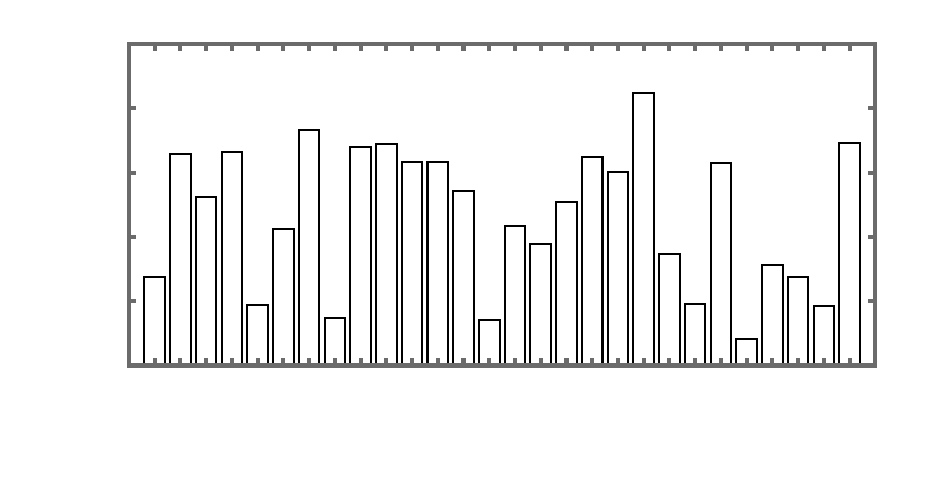
\includegraphics{start}}%
    \gplfronttext
  \end{picture}%
\endgroup
}
      \caption{Average number of infected individuals across the whole of the
      EU28 zone, with data per week and starting country.}
      \label{fig:start}            
   \end{figure}

   \begin{figure}[H]
      \vspace*{1cm}
      \hspace*{-2cm}
      \centering
      \begin{minipage}[t]{.6\textwidth}		
         \vspace{0pt}
         \centering
          \resizebox{\columnwidth}{!}{% GNUPLOT: LaTeX picture with Postscript
\begingroup
  \makeatletter
  \providecommand\color[2][]{%
    \GenericError{(gnuplot) \space\space\space\@spaces}{%
      Package color not loaded in conjunction with
      terminal option `colourtext'%
    }{See the gnuplot documentation for explanation.%
    }{Either use 'blacktext' in gnuplot or load the package
      color.sty in LaTeX.}%
    \renewcommand\color[2][]{}%
  }%
  \providecommand\includegraphics[2][]{%
    \GenericError{(gnuplot) \space\space\space\@spaces}{%
      Package graphicx or graphics not loaded%
    }{See the gnuplot documentation for explanation.%
    }{The gnuplot epslatex terminal needs graphicx.sty or graphics.sty.}%
    \renewcommand\includegraphics[2][]{}%
  }%
  \providecommand\rotatebox[2]{#2}%
  \@ifundefined{ifGPcolor}{%
    \newif\ifGPcolor
    \GPcolorfalse
  }{}%
  \@ifundefined{ifGPblacktext}{%
    \newif\ifGPblacktext
    \GPblacktexttrue
  }{}%
  % define a \g@addto@macro without @ in the name:
  \let\gplgaddtomacro\g@addto@macro
  % define empty templates for all commands taking text:
  \gdef\gplbacktext{}%
  \gdef\gplfronttext{}%
  \makeatother
  \ifGPblacktext
    % no textcolor at all
    \def\colorrgb#1{}%
    \def\colorgray#1{}%
  \else
    % gray or color?
    \ifGPcolor
      \def\colorrgb#1{\color[rgb]{#1}}%
      \def\colorgray#1{\color[gray]{#1}}%
      \expandafter\def\csname LTw\endcsname{\color{white}}%
      \expandafter\def\csname LTb\endcsname{\color{black}}%
      \expandafter\def\csname LTa\endcsname{\color{black}}%
      \expandafter\def\csname LT0\endcsname{\color[rgb]{1,0,0}}%
      \expandafter\def\csname LT1\endcsname{\color[rgb]{0,1,0}}%
      \expandafter\def\csname LT2\endcsname{\color[rgb]{0,0,1}}%
      \expandafter\def\csname LT3\endcsname{\color[rgb]{1,0,1}}%
      \expandafter\def\csname LT4\endcsname{\color[rgb]{0,1,1}}%
      \expandafter\def\csname LT5\endcsname{\color[rgb]{1,1,0}}%
      \expandafter\def\csname LT6\endcsname{\color[rgb]{0,0,0}}%
      \expandafter\def\csname LT7\endcsname{\color[rgb]{1,0.3,0}}%
      \expandafter\def\csname LT8\endcsname{\color[rgb]{0.5,0.5,0.5}}%
    \else
      % gray
      \def\colorrgb#1{\color{black}}%
      \def\colorgray#1{\color[gray]{#1}}%
      \expandafter\def\csname LTw\endcsname{\color{white}}%
      \expandafter\def\csname LTb\endcsname{\color{black}}%
      \expandafter\def\csname LTa\endcsname{\color{black}}%
      \expandafter\def\csname LT0\endcsname{\color{black}}%
      \expandafter\def\csname LT1\endcsname{\color{black}}%
      \expandafter\def\csname LT2\endcsname{\color{black}}%
      \expandafter\def\csname LT3\endcsname{\color{black}}%
      \expandafter\def\csname LT4\endcsname{\color{black}}%
      \expandafter\def\csname LT5\endcsname{\color{black}}%
      \expandafter\def\csname LT6\endcsname{\color{black}}%
      \expandafter\def\csname LT7\endcsname{\color{black}}%
      \expandafter\def\csname LT8\endcsname{\color{black}}%
    \fi
  \fi
  \setlength{\unitlength}{0.0500bp}%
  \begin{picture}(7200.00,5040.00)%
    \gplgaddtomacro\gplbacktext{%
      \colorrgb{0.42,0.42,0.42}%
      \put(1474,704){\makebox(0,0)[r]{\strut{}0}}%
      \colorrgb{0.42,0.42,0.42}%
      \put(1474,1383){\makebox(0,0)[r]{\strut{}3000000}}%
      \colorrgb{0.42,0.42,0.42}%
      \put(1474,2061){\makebox(0,0)[r]{\strut{}6000000}}%
      \colorrgb{0.42,0.42,0.42}%
      \put(1474,2740){\makebox(0,0)[r]{\strut{}9000000}}%
      \colorrgb{0.42,0.42,0.42}%
      \put(1474,3418){\makebox(0,0)[r]{\strut{}12000000}}%
      \colorrgb{0.42,0.42,0.42}%
      \put(1474,4097){\makebox(0,0)[r]{\strut{}15000000}}%
      \colorrgb{0.42,0.42,0.42}%
      \put(1474,4775){\makebox(0,0)[r]{\strut{}18000000}}%
      \colorrgb{0.42,0.42,0.42}%
      \put(1655,484){\makebox(0,0){\strut{}0}}%
      \colorrgb{0.42,0.42,0.42}%
      \put(2636,484){\makebox(0,0){\strut{}10}}%
      \colorrgb{0.42,0.42,0.42}%
      \put(3616,484){\makebox(0,0){\strut{}20}}%
      \colorrgb{0.42,0.42,0.42}%
      \put(4597,484){\makebox(0,0){\strut{}30}}%
      \colorrgb{0.42,0.42,0.42}%
      \put(5577,484){\makebox(0,0){\strut{}40}}%
      \colorrgb{0.42,0.42,0.42}%
      \put(6558,484){\makebox(0,0){\strut{}50}}%
      \colorrgb{0.42,0.42,0.42}%
      \put(176,2739){\rotatebox{-270}{\makebox(0,0){\strut{}Number of people infected}}}%
      \colorrgb{0.42,0.42,0.42}%
      \put(4204,154){\makebox(0,0){\strut{}Weeks passed since first occurence}}%
      \colorrgb{0.42,0.42,0.42}%
      \put(4204,4665){\makebox(0,0){\strut{}}}%
    }%
    \gplgaddtomacro\gplfronttext{%
      \csname LTb\endcsname%
      \put(5804,4602){\makebox(0,0)[r]{\strut{}DE}}%
      \csname LTb\endcsname%
      \put(5804,4382){\makebox(0,0)[r]{\strut{}PT}}%
      \csname LTb\endcsname%
      \put(5804,4162){\makebox(0,0)[r]{\strut{}SE}}%
      \csname LTb\endcsname%
      \put(5804,3942){\makebox(0,0)[r]{\strut{}UK}}%
      \csname LTb\endcsname%
      \put(5804,3722){\makebox(0,0)[r]{\strut{}Other}}%
    }%
    \gplbacktext
    \put(0,0){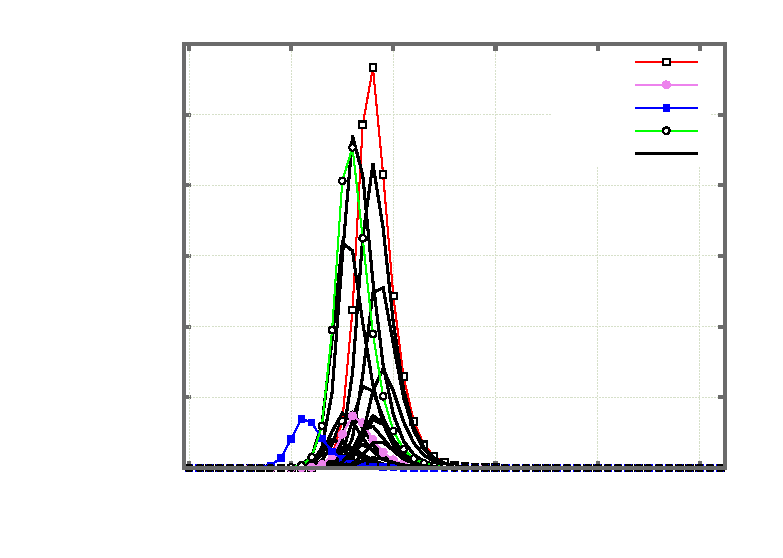
\includegraphics{se}}%
    \gplfronttext
  \end{picture}%
\endgroup
}
          \caption{Infection dynamics with SE as initial target. Note the
          delayed effect for other countries with respect to reaction
          time.}
          \label{fig:se}
      \end{minipage}~\hspace*{1em}
      \begin{minipage}[t]{.6\textwidth}		
         \vspace{0pt}
         \centering
         \resizebox{\columnwidth}{!}{% GNUPLOT: LaTeX picture with Postscript
\begingroup
  \makeatletter
  \providecommand\color[2][]{%
    \GenericError{(gnuplot) \space\space\space\@spaces}{%
      Package color not loaded in conjunction with
      terminal option `colourtext'%
    }{See the gnuplot documentation for explanation.%
    }{Either use 'blacktext' in gnuplot or load the package
      color.sty in LaTeX.}%
    \renewcommand\color[2][]{}%
  }%
  \providecommand\includegraphics[2][]{%
    \GenericError{(gnuplot) \space\space\space\@spaces}{%
      Package graphicx or graphics not loaded%
    }{See the gnuplot documentation for explanation.%
    }{The gnuplot epslatex terminal needs graphicx.sty or graphics.sty.}%
    \renewcommand\includegraphics[2][]{}%
  }%
  \providecommand\rotatebox[2]{#2}%
  \@ifundefined{ifGPcolor}{%
    \newif\ifGPcolor
    \GPcolorfalse
  }{}%
  \@ifundefined{ifGPblacktext}{%
    \newif\ifGPblacktext
    \GPblacktexttrue
  }{}%
  % define a \g@addto@macro without @ in the name:
  \let\gplgaddtomacro\g@addto@macro
  % define empty templates for all commands taking text:
  \gdef\gplbacktext{}%
  \gdef\gplfronttext{}%
  \makeatother
  \ifGPblacktext
    % no textcolor at all
    \def\colorrgb#1{}%
    \def\colorgray#1{}%
  \else
    % gray or color?
    \ifGPcolor
      \def\colorrgb#1{\color[rgb]{#1}}%
      \def\colorgray#1{\color[gray]{#1}}%
      \expandafter\def\csname LTw\endcsname{\color{white}}%
      \expandafter\def\csname LTb\endcsname{\color{black}}%
      \expandafter\def\csname LTa\endcsname{\color{black}}%
      \expandafter\def\csname LT0\endcsname{\color[rgb]{1,0,0}}%
      \expandafter\def\csname LT1\endcsname{\color[rgb]{0,1,0}}%
      \expandafter\def\csname LT2\endcsname{\color[rgb]{0,0,1}}%
      \expandafter\def\csname LT3\endcsname{\color[rgb]{1,0,1}}%
      \expandafter\def\csname LT4\endcsname{\color[rgb]{0,1,1}}%
      \expandafter\def\csname LT5\endcsname{\color[rgb]{1,1,0}}%
      \expandafter\def\csname LT6\endcsname{\color[rgb]{0,0,0}}%
      \expandafter\def\csname LT7\endcsname{\color[rgb]{1,0.3,0}}%
      \expandafter\def\csname LT8\endcsname{\color[rgb]{0.5,0.5,0.5}}%
    \else
      % gray
      \def\colorrgb#1{\color{black}}%
      \def\colorgray#1{\color[gray]{#1}}%
      \expandafter\def\csname LTw\endcsname{\color{white}}%
      \expandafter\def\csname LTb\endcsname{\color{black}}%
      \expandafter\def\csname LTa\endcsname{\color{black}}%
      \expandafter\def\csname LT0\endcsname{\color{black}}%
      \expandafter\def\csname LT1\endcsname{\color{black}}%
      \expandafter\def\csname LT2\endcsname{\color{black}}%
      \expandafter\def\csname LT3\endcsname{\color{black}}%
      \expandafter\def\csname LT4\endcsname{\color{black}}%
      \expandafter\def\csname LT5\endcsname{\color{black}}%
      \expandafter\def\csname LT6\endcsname{\color{black}}%
      \expandafter\def\csname LT7\endcsname{\color{black}}%
      \expandafter\def\csname LT8\endcsname{\color{black}}%
    \fi
  \fi
  \setlength{\unitlength}{0.0500bp}%
  \begin{picture}(7200.00,5040.00)%
    \gplgaddtomacro\gplbacktext{%
      \colorrgb{0.42,0.42,0.42}%
      \put(1474,704){\makebox(0,0)[r]{\strut{}0}}%
      \colorrgb{0.42,0.42,0.42}%
      \put(1474,1383){\makebox(0,0)[r]{\strut{}3000000}}%
      \colorrgb{0.42,0.42,0.42}%
      \put(1474,2061){\makebox(0,0)[r]{\strut{}6000000}}%
      \colorrgb{0.42,0.42,0.42}%
      \put(1474,2740){\makebox(0,0)[r]{\strut{}9000000}}%
      \colorrgb{0.42,0.42,0.42}%
      \put(1474,3418){\makebox(0,0)[r]{\strut{}12000000}}%
      \colorrgb{0.42,0.42,0.42}%
      \put(1474,4097){\makebox(0,0)[r]{\strut{}15000000}}%
      \colorrgb{0.42,0.42,0.42}%
      \put(1474,4775){\makebox(0,0)[r]{\strut{}18000000}}%
      \colorrgb{0.42,0.42,0.42}%
      \put(1655,484){\makebox(0,0){\strut{}0}}%
      \colorrgb{0.42,0.42,0.42}%
      \put(2636,484){\makebox(0,0){\strut{}10}}%
      \colorrgb{0.42,0.42,0.42}%
      \put(3616,484){\makebox(0,0){\strut{}20}}%
      \colorrgb{0.42,0.42,0.42}%
      \put(4597,484){\makebox(0,0){\strut{}30}}%
      \colorrgb{0.42,0.42,0.42}%
      \put(5577,484){\makebox(0,0){\strut{}40}}%
      \colorrgb{0.42,0.42,0.42}%
      \put(6558,484){\makebox(0,0){\strut{}50}}%
      \colorrgb{0.42,0.42,0.42}%
      \put(176,2739){\rotatebox{-270}{\makebox(0,0){\strut{}Number of people infected}}}%
      \colorrgb{0.42,0.42,0.42}%
      \put(4204,154){\makebox(0,0){\strut{}Weeks passed since first occurence}}%
      \colorrgb{0.42,0.42,0.42}%
      \put(4204,4665){\makebox(0,0){\strut{}}}%
    }%
    \gplgaddtomacro\gplfronttext{%
      \csname LTb\endcsname%
      \put(5804,4602){\makebox(0,0)[r]{\strut{}DE}}%
      \csname LTb\endcsname%
      \put(5804,4382){\makebox(0,0)[r]{\strut{}PT}}%
      \csname LTb\endcsname%
      \put(5804,4162){\makebox(0,0)[r]{\strut{}SE}}%
      \csname LTb\endcsname%
      \put(5804,3942){\makebox(0,0)[r]{\strut{}UK}}%
      \csname LTb\endcsname%
      \put(5804,3722){\makebox(0,0)[r]{\strut{}Other}}%
    }%
    \gplbacktext
    \put(0,0){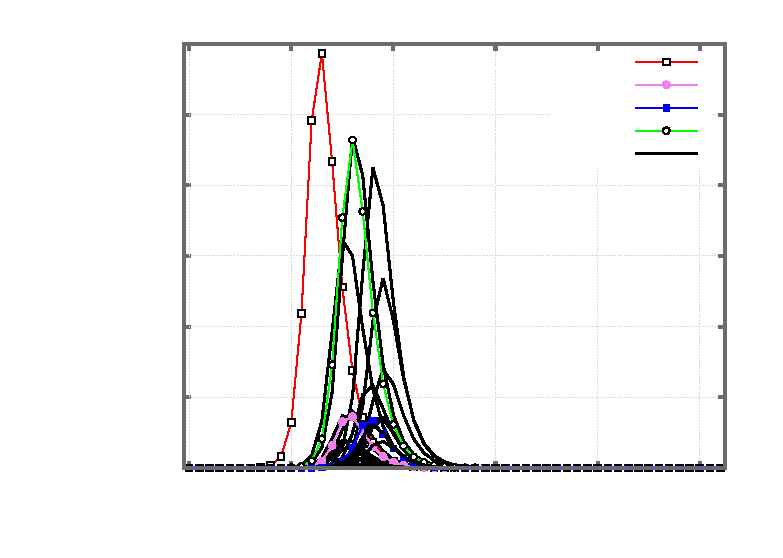
\includegraphics{de}}%
    \gplfronttext
  \end{picture}%
\endgroup
}
         \caption{DE as initial disease host. As with SE, most countries
         follow closely behind as a cluster.}
         \label{fig:de}
      \end{minipage}
   \end{figure}

   As both \cref{fig:se} and \cref{fig:de} signifies however, there can be no conclusive
   result drawn about the pattern of spread, since the high international
   exchange rate of people seems to cause an immediate cluster-reaction,
   independently of where the initial spread takes place. It must however be
   noted that the dynamics certainly can be affected slightly, as both SE and DE
   shift similarily depending on who happens to take on the role of first
   target. Aside from that, other countries display notably similar behaviour between
   the two settings, and are, barring SE and DE, fairly indistinguishable.

   \begin{figure}[H]
      \centering
      \resizebox{.6\textwidth}{!}{% GNUPLOT: LaTeX picture with Postscript
\begingroup
  \makeatletter
  \providecommand\color[2][]{%
    \GenericError{(gnuplot) \space\space\space\@spaces}{%
      Package color not loaded in conjunction with
      terminal option `colourtext'%
    }{See the gnuplot documentation for explanation.%
    }{Either use 'blacktext' in gnuplot or load the package
      color.sty in LaTeX.}%
    \renewcommand\color[2][]{}%
  }%
  \providecommand\includegraphics[2][]{%
    \GenericError{(gnuplot) \space\space\space\@spaces}{%
      Package graphicx or graphics not loaded%
    }{See the gnuplot documentation for explanation.%
    }{The gnuplot epslatex terminal needs graphicx.sty or graphics.sty.}%
    \renewcommand\includegraphics[2][]{}%
  }%
  \providecommand\rotatebox[2]{#2}%
  \@ifundefined{ifGPcolor}{%
    \newif\ifGPcolor
    \GPcolorfalse
  }{}%
  \@ifundefined{ifGPblacktext}{%
    \newif\ifGPblacktext
    \GPblacktexttrue
  }{}%
  % define a \g@addto@macro without @ in the name:
  \let\gplgaddtomacro\g@addto@macro
  % define empty templates for all commands taking text:
  \gdef\gplbacktext{}%
  \gdef\gplfronttext{}%
  \makeatother
  \ifGPblacktext
    % no textcolor at all
    \def\colorrgb#1{}%
    \def\colorgray#1{}%
  \else
    % gray or color?
    \ifGPcolor
      \def\colorrgb#1{\color[rgb]{#1}}%
      \def\colorgray#1{\color[gray]{#1}}%
      \expandafter\def\csname LTw\endcsname{\color{white}}%
      \expandafter\def\csname LTb\endcsname{\color{black}}%
      \expandafter\def\csname LTa\endcsname{\color{black}}%
      \expandafter\def\csname LT0\endcsname{\color[rgb]{1,0,0}}%
      \expandafter\def\csname LT1\endcsname{\color[rgb]{0,1,0}}%
      \expandafter\def\csname LT2\endcsname{\color[rgb]{0,0,1}}%
      \expandafter\def\csname LT3\endcsname{\color[rgb]{1,0,1}}%
      \expandafter\def\csname LT4\endcsname{\color[rgb]{0,1,1}}%
      \expandafter\def\csname LT5\endcsname{\color[rgb]{1,1,0}}%
      \expandafter\def\csname LT6\endcsname{\color[rgb]{0,0,0}}%
      \expandafter\def\csname LT7\endcsname{\color[rgb]{1,0.3,0}}%
      \expandafter\def\csname LT8\endcsname{\color[rgb]{0.5,0.5,0.5}}%
    \else
      % gray
      \def\colorrgb#1{\color{black}}%
      \def\colorgray#1{\color[gray]{#1}}%
      \expandafter\def\csname LTw\endcsname{\color{white}}%
      \expandafter\def\csname LTb\endcsname{\color{black}}%
      \expandafter\def\csname LTa\endcsname{\color{black}}%
      \expandafter\def\csname LT0\endcsname{\color{black}}%
      \expandafter\def\csname LT1\endcsname{\color{black}}%
      \expandafter\def\csname LT2\endcsname{\color{black}}%
      \expandafter\def\csname LT3\endcsname{\color{black}}%
      \expandafter\def\csname LT4\endcsname{\color{black}}%
      \expandafter\def\csname LT5\endcsname{\color{black}}%
      \expandafter\def\csname LT6\endcsname{\color{black}}%
      \expandafter\def\csname LT7\endcsname{\color{black}}%
      \expandafter\def\csname LT8\endcsname{\color{black}}%
    \fi
  \fi
  \setlength{\unitlength}{0.0500bp}%
  \begin{picture}(7200.00,5040.00)%
    \gplgaddtomacro\gplbacktext{%
      \colorrgb{0.42,0.42,0.42}%
      \put(1474,704){\makebox(0,0)[r]{\strut{}0}}%
      \colorrgb{0.42,0.42,0.42}%
      \put(1474,1213){\makebox(0,0)[r]{\strut{}2000000}}%
      \colorrgb{0.42,0.42,0.42}%
      \put(1474,1722){\makebox(0,0)[r]{\strut{}4000000}}%
      \colorrgb{0.42,0.42,0.42}%
      \put(1474,2231){\makebox(0,0)[r]{\strut{}6000000}}%
      \colorrgb{0.42,0.42,0.42}%
      \put(1474,2740){\makebox(0,0)[r]{\strut{}8000000}}%
      \colorrgb{0.42,0.42,0.42}%
      \put(1474,3248){\makebox(0,0)[r]{\strut{}10000000}}%
      \colorrgb{0.42,0.42,0.42}%
      \put(1474,3757){\makebox(0,0)[r]{\strut{}12000000}}%
      \colorrgb{0.42,0.42,0.42}%
      \put(1474,4266){\makebox(0,0)[r]{\strut{}14000000}}%
      \colorrgb{0.42,0.42,0.42}%
      \put(1474,4775){\makebox(0,0)[r]{\strut{}16000000}}%
      \colorrgb{0.42,0.42,0.42}%
      \put(1655,484){\makebox(0,0){\strut{}0}}%
      \colorrgb{0.42,0.42,0.42}%
      \put(2636,484){\makebox(0,0){\strut{}10}}%
      \colorrgb{0.42,0.42,0.42}%
      \put(3616,484){\makebox(0,0){\strut{}20}}%
      \colorrgb{0.42,0.42,0.42}%
      \put(4597,484){\makebox(0,0){\strut{}30}}%
      \colorrgb{0.42,0.42,0.42}%
      \put(5577,484){\makebox(0,0){\strut{}40}}%
      \colorrgb{0.42,0.42,0.42}%
      \put(6558,484){\makebox(0,0){\strut{}50}}%
      \colorrgb{0.42,0.42,0.42}%
      \put(176,2739){\rotatebox{-270}{\makebox(0,0){\strut{}Number of people}}}%
      \colorrgb{0.42,0.42,0.42}%
      \put(4204,154){\makebox(0,0){\strut{}Weeks passed since first occurence}}%
      \colorrgb{0.42,0.42,0.42}%
      \put(4204,4665){\makebox(0,0){\strut{}}}%
    }%
    \gplgaddtomacro\gplfronttext{%
      \csname LTb\endcsname%
      \put(5804,4602){\makebox(0,0)[r]{\strut{}PT: S}}%
      \csname LTb\endcsname%
      \put(5804,4382){\makebox(0,0)[r]{\strut{}PT: I}}%
      \csname LTb\endcsname%
      \put(5804,4162){\makebox(0,0)[r]{\strut{}PT: R}}%
      \csname LTb\endcsname%
      \put(5804,3942){\makebox(0,0)[r]{\strut{}SE: S}}%
      \csname LTb\endcsname%
      \put(5804,3722){\makebox(0,0)[r]{\strut{}SE: I}}%
      \csname LTb\endcsname%
      \put(5804,3502){\makebox(0,0)[r]{\strut{}SE: R}}%
    }%
    \gplbacktext
    \put(0,0){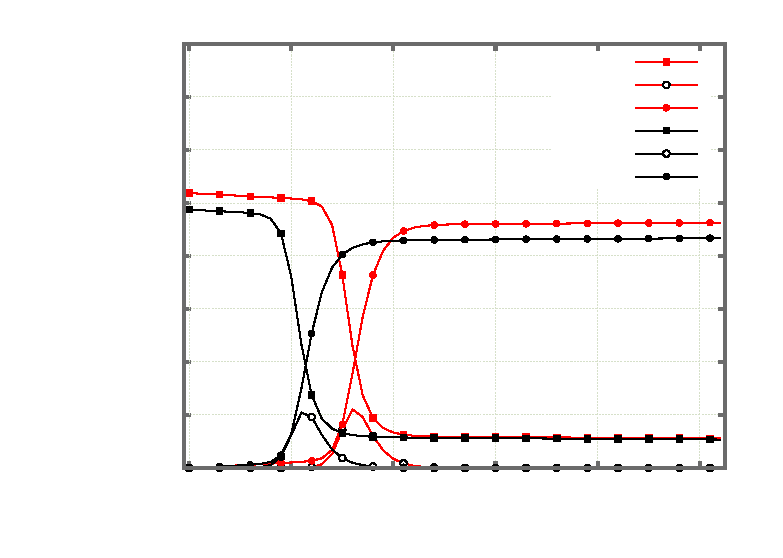
\includegraphics{dyn}}%
    \gplfronttext
  \end{picture}%
\endgroup
}
      \caption{Disease dynamics for SE and PT, where SE is the country of first
      spread. Note the emphasised delay for the rapid increase in infected
      people between the countries. }
      \label{fig:dyn}            
   \end{figure}

   One can in \cref{fig:dyn} witness the aforementioned dynamics of an outbreak,
   where an outbreak in SE causes PT to exhibit its peak rougly six weeks
   later, whereas SE at that rate has nearly eradicated the disease.
   Furthermore, for both separate countries, it is clear that the dynamics are
   uniform in the sense that as soon as the disease has reached its peak, it is
   bound to soon be eradicated.  

   Interestingly enough, every country does in the end reach a state of
   equilibrium, where all derivatives in our model tend to zero. We can however
   not draw any conclusions between the quotas of the different parameters due
   to the travel terms; countries might by chance for example end up with large parts of
   their population pool labelled as a specific category, simply due to a large
   influx of sick individuals -- an obvious limitation to our model with respect
   to reality.  

\section*{Conclusions}
   Of all the countries investigated, there is indeed a bias depending on where
   the first outbreak takes place. There can, however, not be said that this
   causes any direct patterns that would imply any certain connections between
   countries in a more topological regard -- all countries seem intertwined
   such that a disease rather uniformly spreads out across the continent as soon
   as having left the country of first occurrence. 

   The effects are more easily measurable in the case of worst initial country, 
   although the differences that our
   results display can not be said to be of very significant magnitude, since
   all values are of the same order. The difference could although be said to be
   relevant from a more humanitarian perspective, since it in absolute terms sums 
   up to about 80000 people between the respective extremes.
   
   Supposedly the lack of higher variance between countries  is inherent to the 
   choice of parameters, as perhaps it could be
   argued that a vaccination rate of 0.2 percent would be to high for a
   non-lethal disease, and that this would hamper the adequacy compared to an
   actual outcome. 

   The model does nevertheless behave rather realistically on the whole, as the
   apparent dynamics of our disease play in to produce a development that need not
   necessarily be too far from the truth. 

\newpage
\section*{Further research}
  Since the data accounted for is restricted to travel habits by flight, an
  extension to the model could certainly be made with regard to this. The SIR
  model does moreover not account for the dynamics that inherent to a population
  over a longer time span; for example deaths and births, which may be relevant
  to more severe outbreaks. It also does not account for the
  affectance of the disease on infected individual, who may change social habits
  and therefore not spread the disease uniformly throughout the stage of infection.

\begin{thebibliography}{99}
   \bibitem{eurostat}
     Eurostat, 
     \emph{International intra-EU air passenger transport by reporting country and EU
     partner country},
     http://ec.europa.eu/eurostat/data/database, 
     retrieved 2015-09-09.
   \bibitem{rhino}
     Liao, C M, et al.,
     \emph{Probabilistic Transmission Dynamic Model to Assess Indoor Airborne Infection
     Risks},
     Risk Analysis 25 (5): 1097–1107, 
     2005
   \bibitem{lecnotes}
     Tobias Ambjörnsson,
     \emph{Lecture notes, Computational Physics},
     Department of Astronomy and Theoretical Physics,
     Lund University,
     2015.
\end{thebibliography}
\newpage
\appendix
\section*{Code}
      \lstinputlisting[language=Java]{ODEsolver.java}
      \lstinputlisting[language=Java]{DiseaseSpread.java}
      \lstinputlisting[language=Java]{Disease.java}
      \lstinputlisting[language=Java]{Network.java}
      \lstinputlisting[language=Java]{Node.java}
\end{document}

